\section{Methods}

Previous work considers the function of an \gls{esn} to be to connect origins and destinations for a set of demand flows whose distance exceeds vehicle range. This approach is valid but limits the scope of analysis. The approach in this paper considers the function of an \gls{esn} as being to minimize the time-cost imposed by the need to refuel/recharge on drivers of a given vehicle type. For a set of demands defined by origin, destination, and volume, the minimum overall travel time is the overall travel time if all vehicles take their shortest path. This forms a lower bound. Any time spent deviating to a station or at the station can be thought of as a cost imposed by the structure of the \gls{esn}. If travel between an origin and destination is impossible or sufficiently difficult, the driver might pick a different mode (such as air travel) or rent a vehicle of a different fuel type. This forms an upper bound. The method presented here is an optimal \gls{esn} expansion problem which minimizes the travel cost imposed by the \gls{esn}.

\subsection{Supply Network Graphs}

Consider a road network represented by a directed graph $G_R = \{V_R, E_R\}$ where $V_R$ is a set of nodes and $E_R$ is a set of edges. The set of nodes $V_R$ contains places (cities and towns) at the nodes in $V_{P} \subseteq V_R$ and stations at the nodes in $V_{S} \subseteq V_R$. The set of edges $E_R$ contains road links. Drivers may pass by places and stations without stopping and drivers who take the same road path will not necessarily stop at the same stations. Thus, it is useful to transform the graph as in \citep{MirHassani_2013}. Transformed graph $G = \{V, E\}$ contains nodes $V = V_S \cup V_P$ and the edges in $E$ are paths taken along the road network. $E$ contains edges for all pairs in $V$ if the energy consumption required is less than the vehicle \gls{ess} capacity.  Routes along $G_R$ are road-paths. Routes along $G$ are supply-paths. It is not possible for any edge $(i, j) \in E$ to have negative cost thus only simple supply-paths need to be considered.

As is the case in prior work, the method presented requires a set of alternative paths for each origin-destination flow. These paths are found using a k-path routing algorithm \citep{Yen_1971, Qian_2013, Eppstein_1998}. In order to guarantee that the alternative paths are simple paths a second transformation is made. For every place $o \in V_P$ which serves as a demand origin, a level graph $\overline{G}_o = \{V, \overline{E}\}$ is constructed where $\overline{E} \subseteq \hat{E}$ and all edges $(i, j) \in \overline{E}$ lead away from $o$. The graph transformations are demonstrated in Figure \ref{fig:paths}



%In order to facilitate in finding the $k$ shortest simple supply-paths, for each origin $o \in V_P$, a level graph $\overline{G}_o = \{V, \overline{E}\}$ is constructed where $\overline{E} \subseteq \hat{E}$ and all edges $(i, j) \in \overline{E}$ lead away from $o$. Using $\overline{G}$ the $k$ shortest simple supply-paths are found using Yen's method.

\begin{figure}[H]
	\centering
	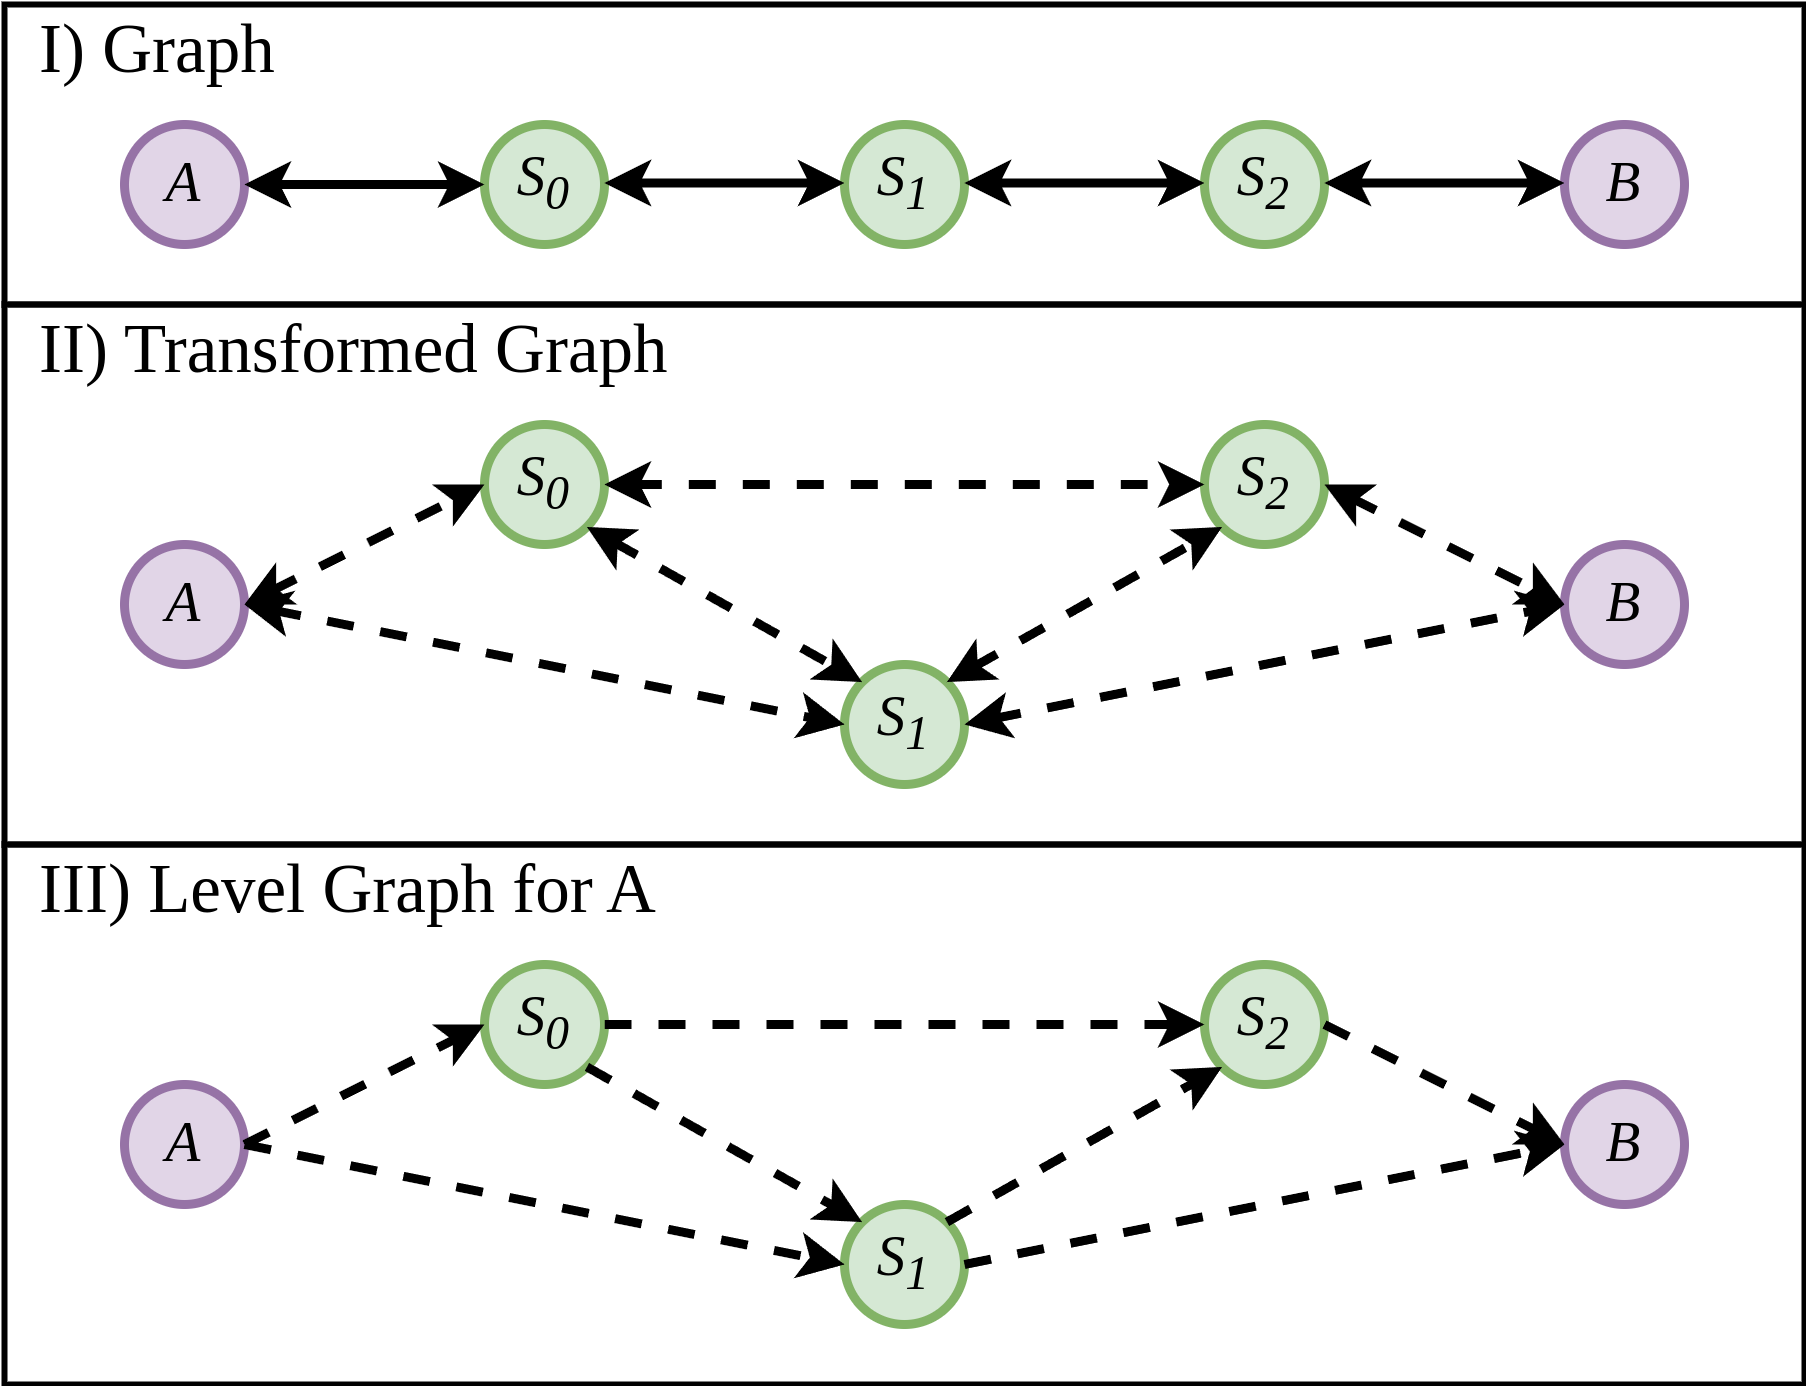
\includegraphics[width = \linewidth]{./figures/formulation/road_charging_paths.png}
	\caption{Graphs for simple vehicular transportation network. Panel I shows a graph $G$ for a section of road from $A$ to $B$ with stations $S_0$, $S_1$, and $S_2$. Panel II shows the transformed graph $\hat{G}$ for a vehicle with sufficient range to reach $S_1$ from $A$ and $B$. Panel III shows the level graph $\overline{G}_A$ for the same vehicle leaving $A$. The simple supply-paths for pair $\langle A, B \rangle$ are $A-S_0-S_1-B$, $A-S_0-S_2-B$, $A-S_1-B$, and $A-S_1-S_2-B$.}
	\label{fig:paths}
\end{figure}

The time cost of edge $(i, j) \in \hat{E}$ is the total trip time. This includes the time required to traverse the edge and the time spent charging at a station before traversing the edge. For a vehicle with a usable \gls{ess} capacity of $\beta$ at node $i$ which contains a charger whose maximum rate is $\alpha$ the time cost for edge $(i, j)$ is

\begin{equation}
	Y^T_{(i, j)} = \tau_{(i, j)} + \begin{cases}
		f_c(\epsilon_{(i, j)}, \beta, \alpha) & \epsilon_{(i, j)} \leq \beta \\
		\infty & \epsilon_{(i, j)} > \beta
	\end{cases}
\end{equation}

where $\tau$ is edge traversal time, $\epsilon$ is edge energy consumption, and $f_c$ is a function relating energy to charging time. Charging is modeled using a CC-CV relationship. The first part of charging is linear and the second part follows an exponential decay function. The time required for a given charge event is

\begin{gather}
	\begin{gathered}
	f_{c}(\epsilon, \beta, \alpha) = \\\begin{cases}
		\frac{\epsilon}{\alpha} & \epsilon \leq \eta\beta \\
		\frac{\eta\beta}{\alpha}\left(1-\ln{\left(1-\frac{\epsilon - \eta\beta}{\beta(1-\eta)}\right)}\right) &  \epsilon > \eta\beta
	\end{cases}
	\end{gathered}
\end{gather}

where $\eta$ is the inflection point separating linear and nonlinear charging. A typical value for $\eta$ will be in the range of 0.7 to 0.8. Charging past $\eta$ will be substantially slower than below $\eta$.

The time-cost of queuing depends on the presence or absence of other vehicles at a station and is modeled at a system level. Queue waiting time is modeled using the M/M/c queuing formula. The expected waiting time in an M/M/c queue is computed as

\begin{gather}
	W_q = f_{q}(\lambda, \mu, c) = \pi_0\frac{\rho(c\rho)^c}{\lambda(1-\rho)^2c!}\label{eq:w_q}\\
	\pi_0=\left[\left(\sum_{k = 0}^{c - 1}\frac{(c\rho)^k}{k!}\right) + \frac{(c\rho)^c}{c!(1 - \rho)}\right]\\
	\rho = \frac{\lambda}{c\mu}
\end{gather}

where $\lambda$ is the mean arrival frequency, $\mu$ is the mean service frequency, $c$ is the number of homogeneous servers, $\rho$ is the ratio of arrival frequency to composite maximum service completion frequency, and $\pi_0$ is the probability of an empty system. The M/M/c formulation assumes exponential distributions for $\lambda$ and $\mu$. One can think of $\rho$ as equivalent to "utilization". Where $\rho$ is low the station has excess capacity and where high the station approaches saturation. $W_q$ approaches infinity as $\rho$ approaches one.

Queue formation is a combinatorial effect. In order to maintain a stable queue length, the rate of vehicle arrivals must match the rate of vehicle departures. This is extremely unlikely over a short time interval and the length of the queue should fluctuate. Over a long enough period, a stable non-zero mean queue length can emerge even when the rate of arrivals is less than the theoretical maximum capacity of the station. This happens because the random sequence of arrivals and departures will, often, produce scenarios where all ports are occupied when the next vehicle arrives. There will be some times when there are no vehicles at the station at all and some times when a long queue exists. \textbf{Scenarios where all ports are occupied are more likely at stations with fewer ports even at identical utilization rates}. This effect is shown in Figure \ref{fig:queue}.

\begin{figure}[H]
	\centering
	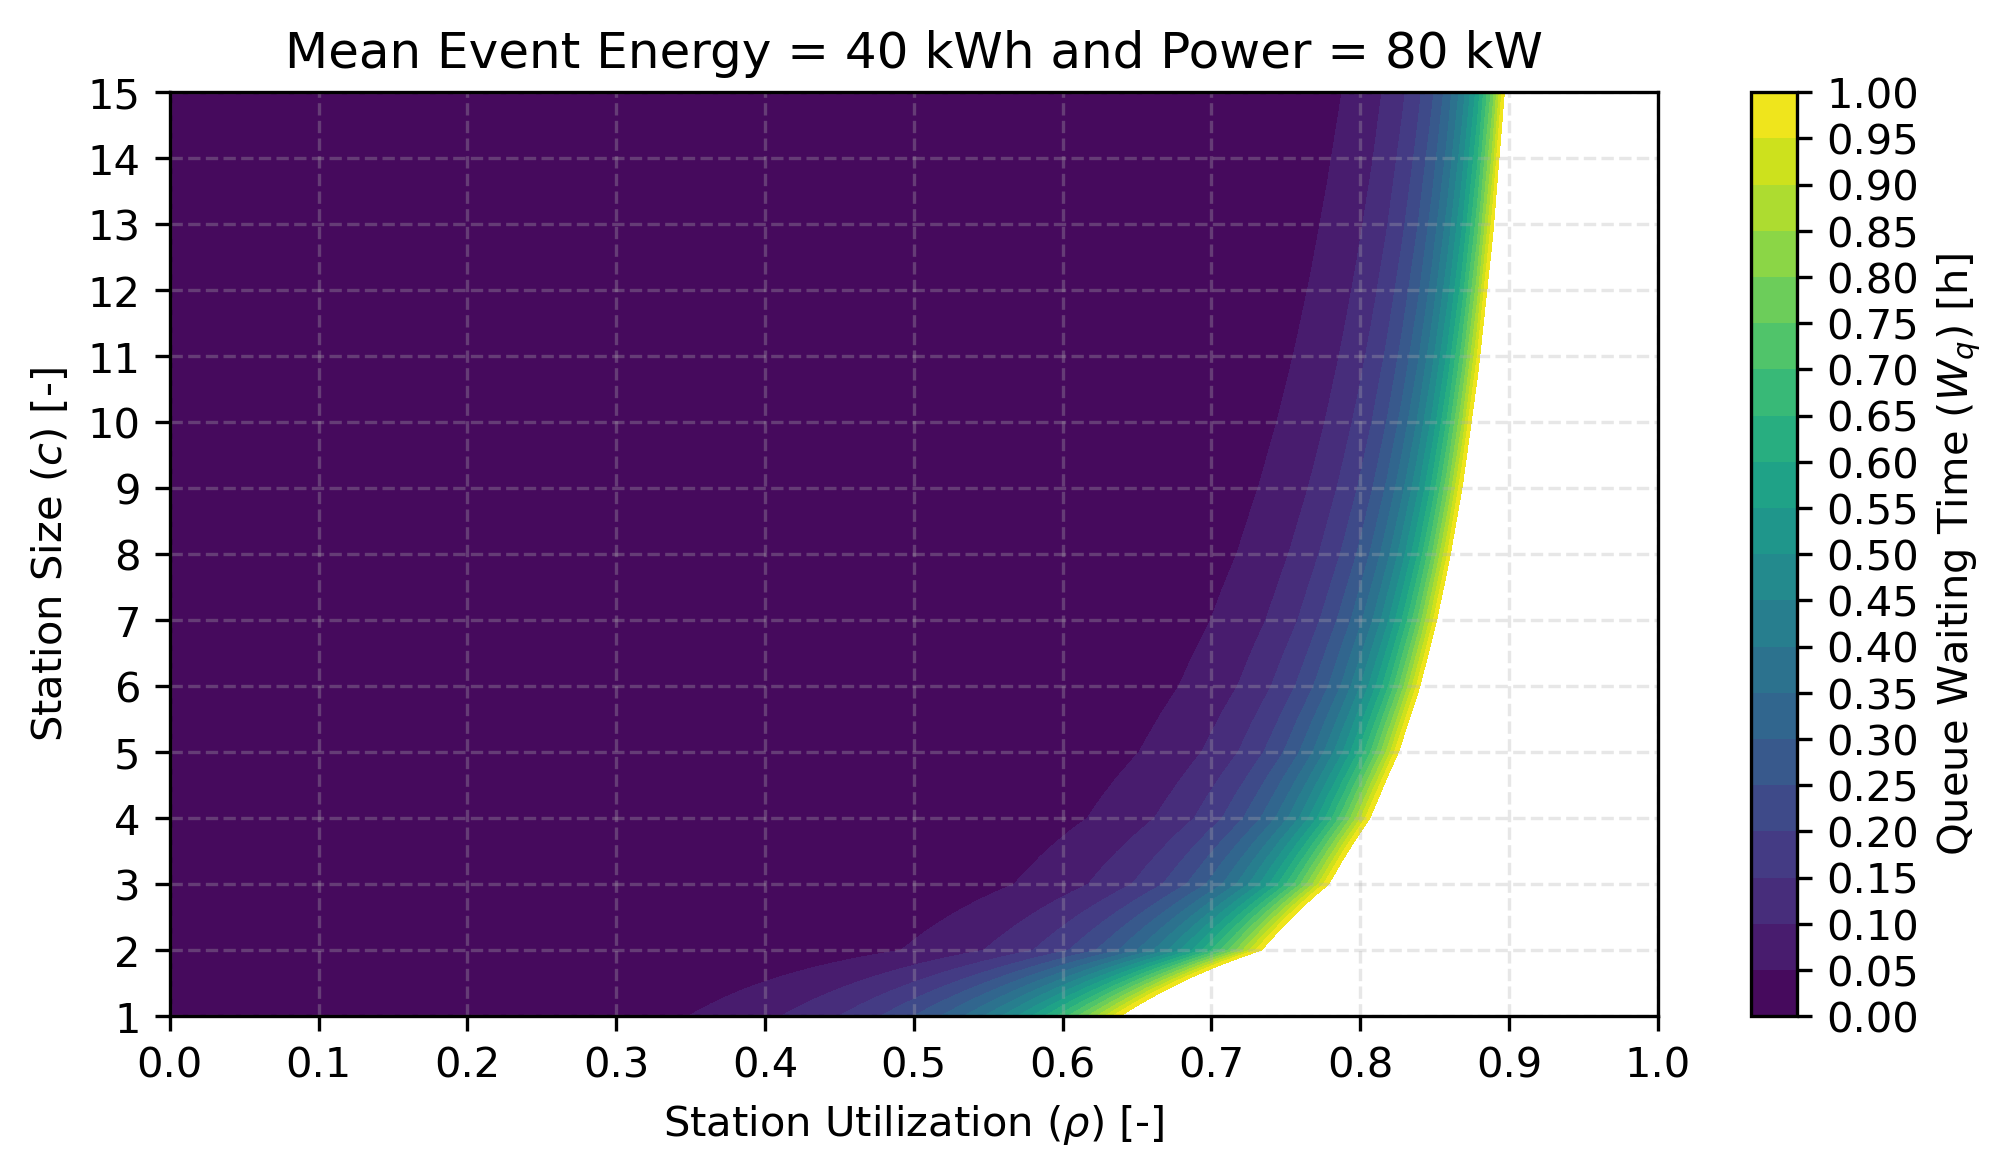
\includegraphics[width = \linewidth]{./figures/formulation/queue.png}
	\caption{Queuing time with M/M/c queue model}
	\label{fig:queue}
\end{figure}

Queuing dynamics mean that larger stations can handle higher utilization rates. As in Figure \ref{fig:queue}, a station with 15 ports can handle a rate of $\rho = 0.8$ before substantial queue formation equivalent to 24 vehicles per hour. A station of 4 chargers can handle a rate of $\rho = 0.6$ before substantial queue formation equivalent to 4.8 vehicles per hour. Thus, larger stations are more efficient on a capacity-per-charger basis with this effect being very substantial below 10 ports and leveling off after 15 ports given current values for mean energy dispensed and charging rate.

\subsection{Formulation}

The purpose of this formulation is to minimize total travel time in the system subject to travel demand. Travel time minimization is accomplished by vehicle routing and charging station provision. For a given origin-destination pair there will, usually, be multiple viable charging paths of different lengths. As demand increases, chargers become increasingly congested leading to queuing time at stations. Queuing delays on shorter paths will push traffic to longer paths. Eventually, queuing will be sufficient to make the charging network no longer beneficial. This point is defined as when the marginal vehicle trip would take as much time using the network as it would take using level 1 charging. The goal is to place chargers and route vehicles to minimize total travel time. As such, each origin-destination pair has a "failure" flow which vehicles can be assigned to and the penalty assigned for this is equal to the travel time with level 1 charging.

Delay at stations is modeled using the outputs of the M/M/c queue formula as previously discussed. Specifically, the outputs are linearized. Stations are initialized with a vector of $m$ binary variables representing possible sizes (e.g. 1 charger, 3 chargers, 5 chargers). The vector of station size binary variables must sum to 1. For each size considered, the M/M/c model returns volumes and delays corresponding to a set of marginal utilization rates $R: |R| = n$. The utilization rates $\rho \in R$ are the bounds of a set of $n - 1$ utilization intervals. Thus, $m$ by $n - 1$ matrices of marginal volumes and marginal delays are created. Additionally, a $m$ by $n$ matrix of unit-interval continuous variables are created and the sum of these variables multiplied by the corresponding marginal volumes must equal the flow passing through the station. the delay at the station is computed by summing the marginal utilization rates multiplied by the marginal delays. In this formulation, travel demand is modeled as a continuous flow in units of vehicles per unit time and accrue at a station simultaneously. This is the same approximation as in the M/M/c queue model.

Optimization uses the following sets:

\begin{itemize}
	\item $G = \{V, E\}$: System graph containing nodes $v \in V$ and edges $(i, j) \in E$. Edge costs are defined by the following sets: \begin{itemize}
		\item $Y^T$: The time required to traverse edge $(i, j)$
		%		\item $Y^E$: The time required to charge at node $i$ to successfully traverse edge $(i, j)$
	\end{itemize}
	\item $O \subseteq V$: Set of origin nodes
	\item $D \subseteq V$: Set of destination nodes
	\item $S \subseteq V$: Set of nodes with charging stations (or the possibility of a station). Stations provide energy to vehicle flows at a given rate. Depending on the utilization level of the station, vehicles may experience delay. The relationship between utilization and delay is linearized using the following sets: \begin{itemize}
		\item $C_s$: Set of possible station sizes at station $s \in S$
		\item $K_{s, c}$: Set of capacity intervals at station $s \in S$ for station size $c \in C_s$
		\item $Y^V$: Set of volumes corresponding to each $c \in C_s$ and $k \in K_s$
		\item $Y^D$: Set of delays corresponding to each $c \in C_s$ and $k \in K_s$ 
		\item $Y^C$: Set of expenditure requirements to install a given number of chargers at a given station.
	\end{itemize}
	\item $\hat{C}$: Maximum number of chargers which can be installed
	\item $Q$: Set of demand tuples of the form $\langle o, d, v, c, \hat{t} \rangle$ where $o$ is the origin, $d$ is the destination, $v$ is the volume, $c$ is the capacity of the \gls{ess} capacity of vehicles, and $\hat{t}$ is the maximum travel time that is acceptable for the given demand. \begin{itemize}
		\item $Y^Q$: Set of time penalties for failing to accommodate flow. Set so that $y^q_q$ is equal to $\hat{t}$ in $q$.
	\end{itemize}
	\item $P$: Set of paths corresponding to each demand $q \in Q$. Paths begin at $o \in O$ and end at $d \in D$. All intermediate nodes $i \in P \setminus \{o, d\}$ must be stations $s \in S$.\begin{itemize}
		\item $P^q$: Paths that correspond to demand $q \in Q$
		\item $P^s$: Paths that include station $s \in S$
	\end{itemize}
	\item $X$: Set of continuous decision variables: \begin{itemize}
		\item $X^Q$: Portion of demand flow not facilitated by the network
		\item $X^P$: Flow volumes along paths
		\item $X^U$: Portion of station capacity intervals utilized
		\item $X^V$: Volume seen at station
		\item $X^D$: Queuing delay seen at station
	\end{itemize}
	\item $U$: Set of integer decision variables: \begin{itemize}
		\item $U^S$: Booleans for station sizes corresponding to $S$ and $C$
	\end{itemize}
\end{itemize}


The objective of the optimization is

\begin{gather}
	\begin{gathered}
	\min_{\overline{X},\overline{U}}\quad \underbrace{\sum_{q \in Q} x^q_qy^q_q}_{\text{Penalty Time}} + \underbrace{\sum_{q \in Q}\sum_{P^q \in P}\sum_{p \in P^q}\sum_{(i, j) \in p} x^p_py^t_{(i, j)}}_{\text{Edge Traversal Time}} \\+ \underbrace{\sum_{s \in S}\sum_{c \in C_s}
		\sum_{k \in K_{s, c}} u^s_{s, c}x^u_{s, c, k}y^d_{s, c, k}}_{\text{Queuing Time}} \label{eq:tm:obj}
	\end{gathered}
\end{gather}

subject to

\begin{gather}
	Q[v] - x^q_q - \sum_{p \in P^q}x^p_p = 0 \quad \forall q \in Q \label{eq:tm:flow_dem} \\
	\sum_{p \in P^s} x^p_p - \sum_{c \in C_s}
	\sum_{k \in K_{s, c}} u^s_{s, c}x^u_{s, c, k}y^v_{s, c, k} = 0 \quad \forall s \in S \label{eq:tm:flow_cons} \\
	x^u_{s, c, k} - u^s_{s, c} \leq 0 \quad \forall s \in S, \ \forall c \in C_s,\ \forall k\in K_{s, c} \label{eq:tm:sz_int} \\
	\sum_{c \in C_s} u^s_{s, c} - 1 = 0 \quad \forall s \in S \label{eq:tm:chg_unity} \\
	\sum_{s \in S}\sum_{c \in C_s} y^c_{s, c}u^s_{s, c} - \hat{C} \leq 0 \label{eq:tm:chg_tot}
\end{gather}

The objective function \eqref{eq:tm:obj} minimizes total travel time in three terms. The first term is the time penalties accrued for failing to accommodate demand. The theory is that, without dedicated charging infrastructure, vehicles could, theoretically, complete the trip using level 1 charging but this would be very slow if the trip is beyond full-charge range. The second term is the time spent driving along edges and charging to drive along edges. The third term is the time spend queuing for a charger. Constraint \eqref{eq:tm:flow_dem} forces the sum of flows and un-accommodated flows to be equal to total demand. Constraint \eqref{eq:tm:flow_cons} forces the sum of utilization intervals at a station to be equal to the sum of flows which pass through the station. Constraint \eqref{eq:tm:sz_int} forces station utilization to only accrue for the selected station size. Constraint \eqref{eq:tm:chg_unity} forces only one station size to be selected per station and \eqref{eq:tm:chg_tot} limits the total number of chargers in the network. This formulation can be used for two varieties of analysis.

\begin{description}
	\item [Performance of Current System:] If all Booleans in $U^S$ are fixed to reflect an existing system, the result of the optimization will be the best possible performance of the existing system for a given demand level.
	\item [Optimal Expansion:] If the Booleans in $U^S$ are allowed to be changed by the optimizer, the result of the optimization will be the best possible allocation of resources to facilitate travel for a given demand level.
\end{description}

Taking the example simple network from Figure \ref{fig:paths}, one can intuit that, if each additional charger at each station is of the same cost ($Y^C_{s, c} = 1\ \forall s\in S,\ c\in C_s$), the optimal solution will be to place all available resources at the central station $S_1$ because only it can be reached from both $A$ and $B$. Doing so will give the greatest benefit in terms of queuing efficiency. The costs of adding and removing chargers may scale in a nonlinear manner. It is easy to imagine a scenario where a network operator finds it easier to remove an existing charger than to install a new charger. Re-allocating equipment between stations in a network is unlikely to be a net-zero cost operation. In such a case, the optimal solution may or may not be altered.